\documentclass{../../presentation}

\title{Άλγεβρα Α Λυκείου}
\subtitle{Συστήματα Συντεταγμένων}
\author[Λόλας]{Κωνσταντίνος Λόλας}
\date{\today}

\begin{document}

\frame{\titlepage}

\section{Θεωρία}

\begin{frame}{Ζωγραφική!!!!!}
  Χρειαζόμαστε Καμβά! Μπορείτε να ευχαριστήσετε τον Descartes για αυτό.
  \begin{figure}
    \centering
    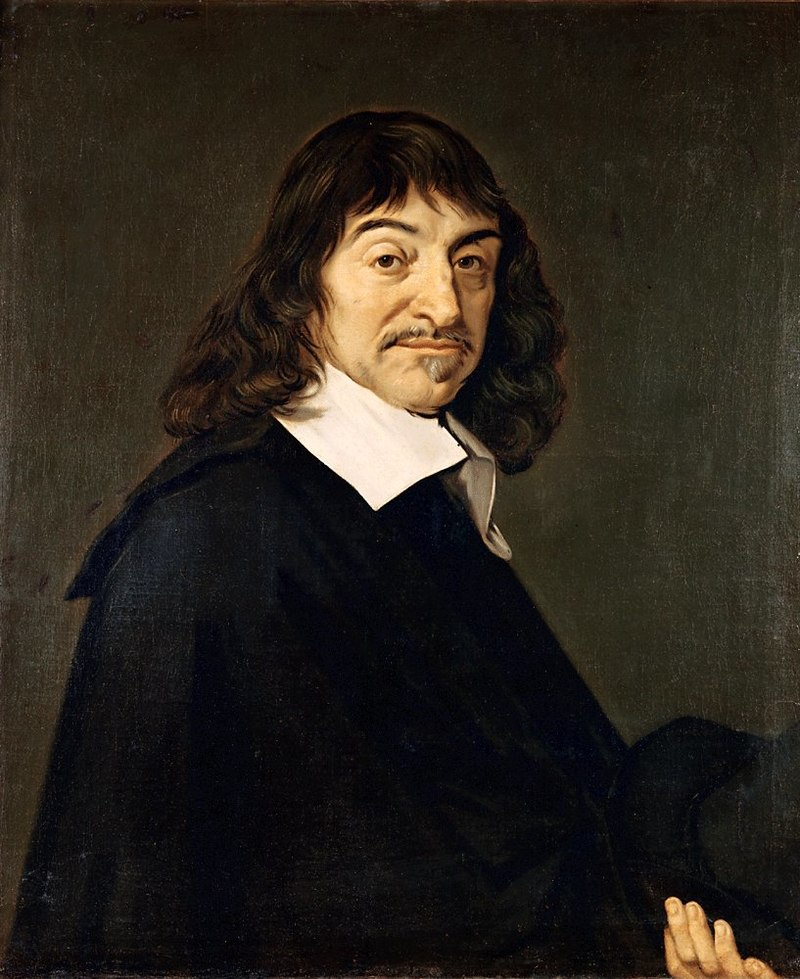
\includegraphics[width=0.5\textwidth]{images/Descartes}
    \caption{René Descartes - Πατέρας της Αναλυτικής Γεωμετρίας}
  \end{figure}
\end{frame}

\begin{frame}{Βάφτιση!}
  \begin{block}{Άξονες}
    Στο επίπεδο σχηματίζουμε δύο κάθετους άξονες $x'x$ και $y'y$ με αρχή το σημείο $O$. Ο άξονας $x'x$ ονομάζεται άξονας των τετμημένων ή άξονας των $x$ και ο άξονας $y'y$ άξονας των τεταγμένων ή άξονας των $y$.
  \end{block}
  \begin{block}{Σημεία}
    Κάθε σημείο $A$ του επιπέδου προσδιορίζεται από δύο πραγματικούς αριθμούς $(x,y)$, οι οποίοι ονομάζονται συντεταγμένες του σημείου $A$. Ο αριθμός $x$ ονομάζεται τετμημένη του σημείου $A$ και είναι η απόσταση από τον άξονα $y$ και ο αριθμός $y$ ονομάζεται τεταγμένη του σημείου $A$ και είνα η απόσταση από τον άξονα $x$.
  \end{block}
\end{frame}

\begin{frame}{Και λίγο ακόμα}
  \begin{block}{Καρτεσιανό Σύστημα Συντεταγμένων}
    Η προηγούμενη διάταξη των δύο αξόνων και των σημείων του επιπέδου ονομάζεται καρτεσιανό σύστημα συντεταγμένων στο επίπεδο.
  \end{block}
  Προφανώς και υπάρχουν και άλλα συστήματα συντεταγμένων όπως
  \begin{itemize}
    \item Πολικό σύστημα συντεταγμένων
    \item Σφαιρικό σύστημα συντεταγμένων
    \item Κυλινδρικό σύστημα συντεταγμένων (δεν ξέρω τα άλλα...)
  \end{itemize}
\end{frame}

\begin{frame}{Πάνω δεξιά, όχι όχι, κάτω αριστερά!}
  Τεταρτημόρια!
  \begin{center}
    \begin{tikzpicture}[scale=1]
      % Draw axes
      \draw[->] (-3,0) -- (3,0) node[right] {$x$};
      \draw[->] (0,-3) -- (0,3) node[above] {$y$};

      % Draw quadrant labels
      \node at (1.5,1.5) {I (+,+)};
      \node at (-1.5,1.5) {II (-,+)};
      \node at (-1.5,-1.5) {III (-,-)};
      \node at (1.5,-1.5) {IV (+,-)};

      % Draw origin
      \node[below left] at (0,0) {$O$};
    \end{tikzpicture}
  \end{center}
\end{frame}

\begin{frame}{Quizes}
  \begin{itemize}[<+->]
    \item Τι καταπληκτικό έχουν τα σημεία του άξονα $x$;
    \item Τι καταπληκτικό έχουν τα σημεία του άξονα $y$;
    \item Πώς κατασκευάζεται το συμμετρικό ενός σημείου:
          \begin{itemize}[<+->]
            \item Σχετικά με τον άξονα $x$;
            \item Σχετικά με τον άξονα $y$;
            \item Σχετικά με την ευθεία $y=x$;
            \item Σχετικά με την αρχή των αξόνων;
          \end{itemize}
  \end{itemize}
\end{frame}

\begin{frame}{Αποστάσεις}
  \begin{itemize}[<+->]
    \item Κατακότυφη απόσταση σημείων \onslide<2-> $d=|y_1-y_2|$
    \item Οριζόντια απόσταση σημείων \onslide<3-> $d=|x_1-x_2|$
    \item Απόσταση σημείων \onslide<4-> $d=\sqrt{(x_2-x_1)^2+(y_2-y_1)^2}$
  \end{itemize}
\end{frame}

\moodle

\section{Ασκήσεις}

\exercises

\begin{askisi}
  Να βρείτε τις τιμές του $α$, για τις οποίες το σημείο $Α(3α-6,2α+8)$ βρίσκεται:
  \begin{itemize}
    \item Στον άξονα $x$.
    \item Στον άξονα $y$.
    \item Στο δεύτερο τεταρτημόριο.
  \end{itemize}
\end{askisi}

\begin{askisi}
  Να βρείτε το συμμετρικό του σημείου $A(2,-1)$, ως προς:
  \begin{itemize}
    \item Τον άξονα $x$.
    \item Τον άξονα $y$.
    \item Την διχοτόμο των γωνιών $\widehat{xOy}$ και $\widehat{x'Oy'}$.
    \item Την αρχή των αξόνων.
  \end{itemize}
\end{askisi}

\begin{askisi}
  Να βρείτε την απόσταση των σημείων:
  \begin{itemize}
    \item $A(-1,2)$ και $B(-3,-1)$.
    \item $Ο(0,0)$ και $A(3,4)$.
    \item $A(2,1)$ και $B(2,5)$.
    \item $A(-1,4)$ και $B(3,4)$.
  \end{itemize}
\end{askisi}

\begin{askisi}
  Έστω το σημείο $Β(0,1)$. Να βρείτε το σημείο $A$ στον άξονα $x$ ώστε το εμβαδόν $Ε$ του τριγώνου $OAB$ να είναι ίσο με $4$.
\end{askisi}

\end{document}